% (c) Jeremy Jacob
% This file is made available for educational purposes
% It may not be distributed for profit, or without this header.

% Altered by Daniel Brown.

\documentclass[aspectratio=1610]{beamer}
\usepackage[T1]{fontenc}
\usepackage[british]{babel}
\usepackage[sc]{mathpazo}
\usepackage[scaled=0.9]{helvet}
\usepackage{courier,textcomp,amsmath,listings, color}
\newcommand{\code}[1]{\texttt{#1}}

% THEME SET UP
% University colours
\definecolor{UoYgreen}{cmyk}{0.82,0.00,0.64,0.70} % Pantone 567
\definecolor{UoYblue} {cmyk}{1.00,0.72,0.00,0.32} % Pantone 281
% Departmental colours
\definecolor{UoYCSbrightgreen}{cmyk}{0.46,0.17,1.00,0.01}
\definecolor{UoYCSyellowgreen}{cmyk}{0.16,0.02,0.51,0.00}
\definecolor{UoYCSgrey}       {cmyk}{0.00,0.00,0.00,0.60}
\definecolor{UoYCSblue}       {cmyk}{0.99,0.68,0.28,0.10}

\usetheme[secheader]{Boadilla}
\usecolortheme[named=UoYCSblue]{structure}
\setbeamertemplate{navigation symbols}{} %removes navigation buttons

% CODE HIGHLIGHTING COLOURS SET UP
% Set up for C#, Credit: http://tex.stackexchange.com/questions/124953/syntax-highlighting-in-listings-for-c-that-it-looks-like-in-visual-studio
%\setmonofont{Consolas} %to be used with XeLaTeX or LuaLaTeX
\definecolor{bluekeywords}{rgb}{0,0,1}
\definecolor{greencomments}{rgb}{0,0.5,0}
\definecolor{redstrings}{rgb}{0.64,0.08,0.08}
\definecolor{xmlcomments}{rgb}{0.5,0.5,0.5}
\definecolor{types}{rgb}{0.17,0.57,0.68}

\lstset
{
  language=Ruby,
  captionpos=b,
  %numbers=left,
  %numberstyle=\tiny,
  frame=lines,
  showspaces=false,
  showtabs=false,
  breaklines=true,
  showstringspaces=false,
  breakatwhitespace=true,
  escapeinside={(*@}{@*)},
  commentstyle=\color{greencomments},
  morekeywords={partial, var, value, get, set},
  keywordstyle=\color{bluekeywords},
  stringstyle=\color{redstrings},
  basicstyle=\ttfamily\small,
}

%Presentation information
\title[EpsilonGit]{EpsilonGit - Advanced Querying of Git Repositories}
\author[DTB]{Daniel Brown}
\institute[UoY, CS]{The University of York, Department of Computer Science}
\date{\today}

\begin{document}
\frame{\titlepage}

\section{Explanation of Research Problem} %Section title on top of each slide
\begin{frame}
\frametitle{What is Git?}
\begin{enumerate}
	\item Distributed Version Control Software
	\item Powers popular GitHub social coding platform (96th most popular site worldwide)
	\item Millions of users managing millions of repositories
	\item A growing platform...
	\begin{figure}[H]
		\centering
		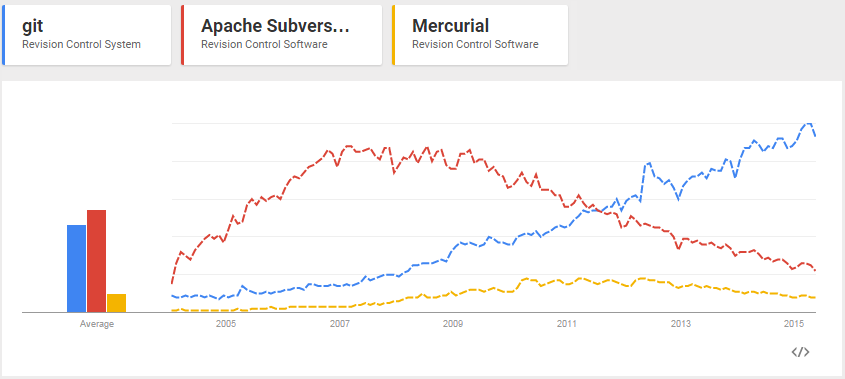
\includegraphics[width=300px]{images/git-google-trends.png}
		\caption{The growth of Git relative to other popular version control systems (Google Trends)}
	\end{figure} 
\end{enumerate}
%https://github.com/blog/1724-10-million-repositories
\end{frame}

\begin{frame}
\frametitle{How do developers use Git?}
\begin{enumerate}
	\item (Sensible) developers make source control the cornerstone of their development
	\item Small, frequent commits in feature branches
	\item Accepting pull requests in Open Source communities
	\item In large-scale projects such as the Linux Kernal, The Roslyn C\# Compiler
	\item In small scale, entirely local repositories
\end{enumerate}
\end{frame}

\begin{frame}
\frametitle{How do developers query \& analyse their git repositories?}
\begin{enumerate}
	\item In short, most don't.
	\item Due in part to lack of software solutions to help
	\item Out of the box the best tool for the job is \code{git log}
\end{enumerate}

\begin{figure}[H]
	\centering
	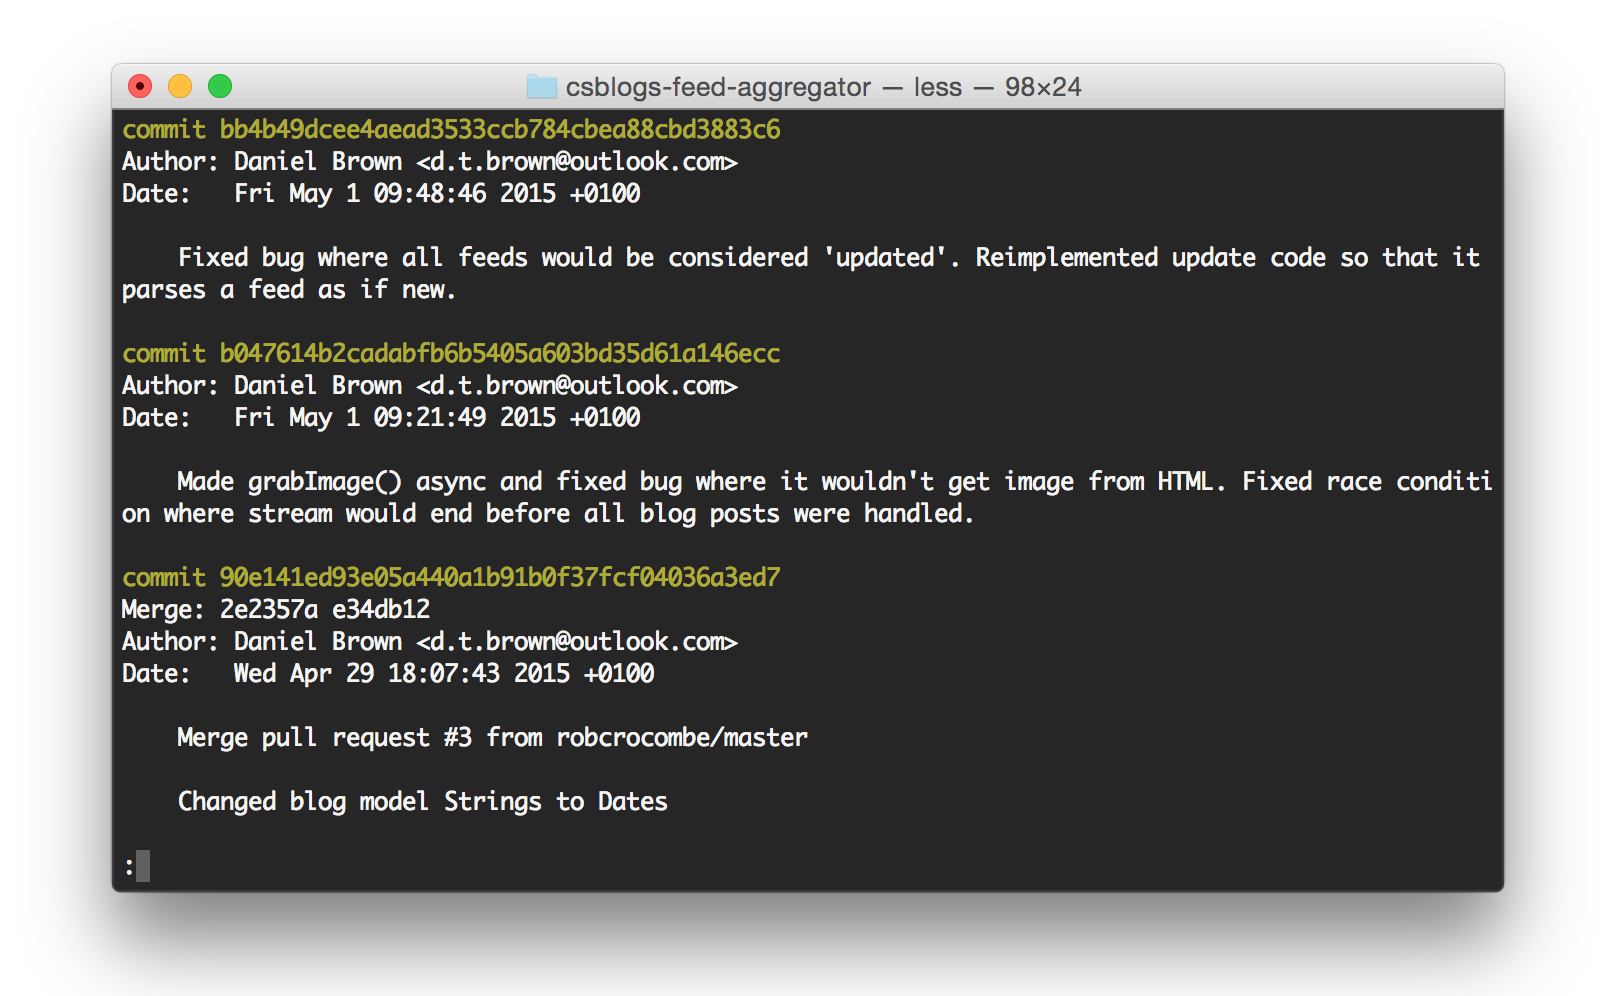
\includegraphics[width=250px]{images/git-log.png}
	\caption{The output of the \code{git log} command}
\end{figure} 
\end{frame}

\begin{frame}
\frametitle{How do developers query \& analyse their git repositories?}
\begin{enumerate}
	\item GitHub provides some additional statistics 
	\item For developers not using GitHub there is GitInspector or GitStat, they both do roughly the same thing
	\item \beamergotobutton{\href{https://www.youtube.com/watch?t=36\&v=NjUuAuBcoqs}{Gource Git Visualization Video on YouTube}}\vspace{10 mm}
\end{enumerate}
\begin{figure}[H]
	\centering
	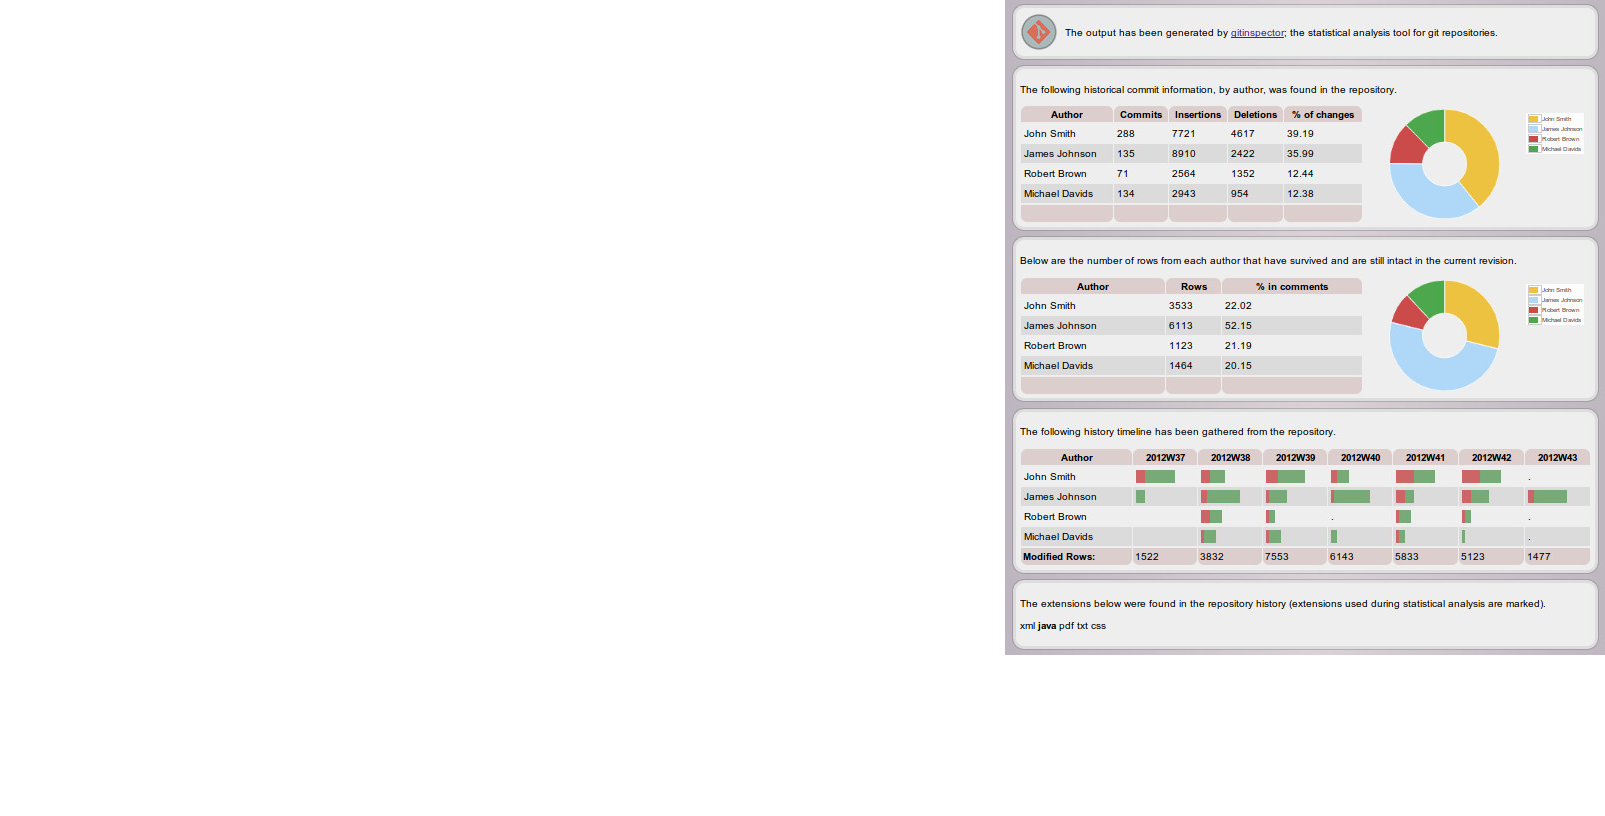
\includegraphics[width=230px]{images/github-analytics-gitinspector-analytics.png}
	\caption{Left: GitHub repository statistics, Right: The HTML output of GitInspector}
\end{figure} 
\end{frame}

\begin{frame}[containsverbatim]
\frametitle{Pain Points / Oppertunities}
\begin{enumerate}
	\item You get the data provided by the queries GitHub/GitInspector makes available and nothing more
	\item No advanced queries. Can't write a query such as the one shown in Listing \ref{lst:exampleCode}
	\item You get the data in the formats provided by GitHub/GitInspector and nothing more
\end{enumerate}

\begin{lstlisting}[caption=An advanced Git query in EOL, label=lst:exampleCode]
File.all.select(f|f.lines > 200 and 
  (f.lastModifiedBy = "joe@foo.com" or f.lastModifiedDay = "Wednesday"))
  \end{lstlisting}
\end{frame}

\begin{frame}
\frametitle{Proposed Solution}
\begin{enumerate}
	\item A driver for Epsilon through the Epsilon Model Connectivity Layer
	\item This allows for all the cool stuff Epsilon does to work on Git
\end{enumerate}
\begin{figure}[H]
	\centering
	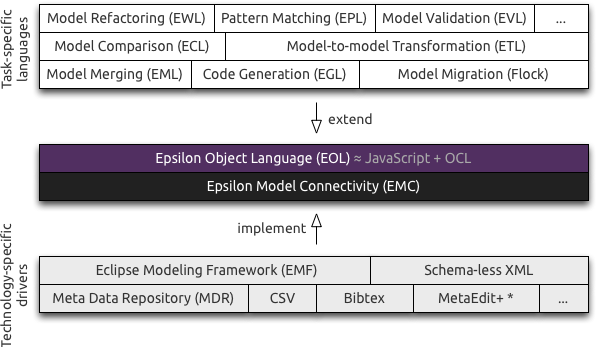
\includegraphics[width=290px]{images/epsilon-architecture}
	\caption{The Architecture of Epsilon}
\end{figure} 
\end{frame}

\section{Literature Review}
\begin{frame}
\frametitle{Literature Review}
\begin{enumerate}
	\item Literature review undertaken to:
		\begin{enumerate} 
			\item determine what could be done that was novel
			\item find alternative solutions
			\item see what existing research could be built upon
		\end{enumerate}
	\item Found that no-one has published any papers about a model-driven engineering approach to interfacing with git or any VCS
	\item The metamodel for git hasn't been formalised (though object model is well understood)
	\item Lots of information about MDE (with Epsilon) available 
\end{enumerate}
\end{frame}

\section{Plan to conduct work}

\begin{frame}
\frametitle{Planning my Research \& Planning}	
\begin{enumerate}
	\item Literature Review
	\item Small scale tests (EMF generation vs Epsilon Model Connectivity etc.)
	\item Plan implementation based on results of tests
\end{enumerate}	
\end{frame}


\begin{frame}
\frametitle{Planning Implementation Development}	
\begin{enumerate}
	\item Initial research amd discussion with supervisor suggests EMC is the way to go
	\item TDD, Integration Tests etc
	\item Interface with Git Object Model via EMC interfaces
	\item Agile is the best buzzword
\end{enumerate}	
\end{frame}

\begin{frame}
\frametitle{Planning report, presentation \& workshop}	
\begin{enumerate}
	\item Feature freeze in mid-July. Implementation finish by August.
	\item Final four weeks dedicated to writing report/workshop/presentation
	\item Build on this presentation. Build on notes collected in GitHub Wiki over course of project.
	\begin{figure}[H]
		\centering
		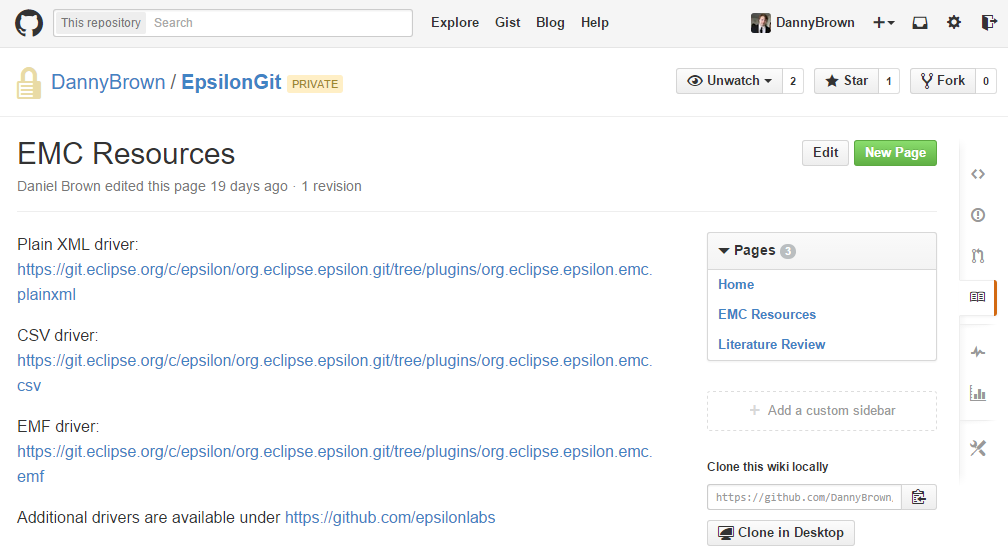
\includegraphics[width=290px]{images/github-wiki}
		\caption{The EpsilonGit GitHub wiki is used to keep track of information to use in reports}
	\end{figure} 
\end{enumerate}	
\end{frame}


\section{Plan to evaluate work}
\begin{frame}
\frametitle{How will EpsilonGit be evaluated?}
\begin{enumerate}
	\item No direct competitor to compare against so...
	\item Compare against the existing git analysis software mentioned previously (speed, range of features, ease of use, etc.)
	\item Compare with other Epsilon drivers (speed)
	\item Compare against aims and objectives of project
\end{enumerate}	
\end{frame}

\section{Finishing up}
\begin{frame}
\frametitle{Thanks for listening}
\begin{figure}[H]
	\centering
	
\includegraphics[width=250px]{images/epsilon-git.png}
\end{figure} 
\begin{enumerate}
	\item I will now answer any questions
	\item You can read more about the project as it progresses at \beamergotobutton{\href{http://dannybrown.net}{dannybrown.net}}\vspace{10 mm}
\end{enumerate}
\end{frame}

\end{document}
